\documentclass[12pt]{article}

% ------------------------------------------------------------
% Fonts and Typography
% ------------------------------------------------------------

\usepackage{fontspec}
\setmainfont{Latin Modern Roman}

\usepackage{microtype}

% ------------------------------------------------------------
% Page Layout
% ------------------------------------------------------------

\usepackage{geometry}
\geometry{margin=1in}

\usepackage{setspace}
\onehalfspacing

% ------------------------------------------------------------
% Mathematics
% ------------------------------------------------------------

\usepackage{amsmath}
\usepackage{amssymb}
\usepackage{amsthm}
\usepackage{mathtools}

% ------------------------------------------------------------
% Diagrams
% ------------------------------------------------------------

\usepackage{tikz}
\usetikzlibrary{arrows.meta, positioning, calc, shapes.geometric, decorations.pathreplacing, fit, backgrounds, matrix, cd}
\usepackage{pgfplots}
\pgfplotsset{compat=1.18}

% ------------------------------------------------------------
% Tables
% ------------------------------------------------------------

\usepackage{booktabs}
\usepackage{array}

% ------------------------------------------------------------
% Hyperlinks
% ------------------------------------------------------------

\usepackage{hyperref}

\hypersetup{
colorlinks=true,
linkcolor=black,
citecolor=black,
urlcolor=blue
}

% ------------------------------------------------------------
% Theorem Environments
% ------------------------------------------------------------

\newtheorem{theorem}{Theorem}[section]
\newtheorem{corollary}[theorem]{Corollary}
\newtheorem{lemma}[theorem]{Lemma}
\newtheorem{proposition}[theorem]{Proposition}
\newtheorem{definition}[theorem]{Definition}
\newtheorem{remark}[theorem]{Remark}

% ------------------------------------------------------------
% Operators
% ------------------------------------------------------------

\DeclareMathOperator{\rank}{rank}
\DeclareMathOperator{\im}{im}
\DeclareMathOperator{\Hom}{Hom}
\DeclareMathOperator{\Ob}{Ob}
\DeclareMathOperator{\colim}{colim}
\DeclareMathOperator{\sh}{Sh}

% ------------------------------------------------------------
% Title
% ------------------------------------------------------------

\title{
The Coordination Engine:\\
\large Civilization as an Error-Correcting System
}
\author{Flyxion}
\date{\today}


% ------------------------------------------------------------
% Document
% ------------------------------------------------------------

\begin{document}

\maketitle

\begin{abstract}

A growing body of cultural commentary argues that civilization is entering an inevitable phase of collapse. According to this view, the agricultural revolution initiated a long historical mistake: the abandonment of small egalitarian bands for large hierarchical societies that generate alienation, inequality, and systemic fragility. Modern technological civilization, despite its conveniences, is portrayed as psychologically corrosive and structurally unstable.

This essay argues that such interpretations fundamentally mischaracterize the nature of civilization itself. Civilization is not a pathological deviation from human nature but an evolving coordination system that enables large-scale cooperation among strangers across time and space. Many of the problems attributed to civilization arise not from its existence but from transitional phases in its development. Periods of institutional instability frequently accompany major shifts in the technological and informational infrastructure that supports social organization.

What appears to some observers as civilizational decline is more plausibly interpreted as a phase transition in the architecture of coordination. Such transitions are mathematically characterized by bifurcations in the parameter space of institutional dynamics, in which old equilibria become unstable and new attractors emerge. The formal tools developed here---spanning information-theoretic error correction, replicator dynamics, sheaf-theoretic knowledge integration, categorical coordination functors, and thermodynamic entropy production---provide a unified framework within which this interpretation can be rendered precise.

The challenge of the present moment is therefore not to retreat from civilization but to understand how its emerging forms of organization can better align with human psychological and social needs while preserving the distributed error-correcting capacities that make long-term knowledge accumulation possible.

\end{abstract}

\newpage
\tableofcontents

\newpage
\section{Introduction}

It has become increasingly common to hear the claim that civilization is approaching collapse. Rising political polarization, ecological strain, fragile supply chains, and widespread psychological distress are often cited as evidence that the entire civilizational project has reached its limits. In this narrative, modern society is not simply experiencing temporary turbulence but revealing a deeper structural flaw that has been present since the earliest stages of organized settlement.

The argument often begins with a contrast between prehistoric hunter--gatherer societies and agricultural civilizations. Small nomadic bands are depicted as socially cohesive and psychologically grounded, while the emergence of agriculture is interpreted as a historical compromise that introduced hierarchy, property, territorial conflict, and institutionalized inequality. From this perspective, modern technological society represents the culmination of a long trajectory in which stability and convenience were purchased at the cost of autonomy, community, and meaning.

Such interpretations capture genuine anxieties about contemporary life. Many people experience modern institutions as distant, opaque, and difficult to influence. Economic and technological systems appear increasingly complex, and the scale of global interdependence can make societies seem fragile in the face of disruption. Yet these observations do not necessarily support the conclusion that civilization itself is fundamentally pathological. To diagnose a system as failing, one must first possess a model of what the system is for and how it operates. The collapse narrative, we shall argue, lacks such a model.

This essay proposes a different interpretation grounded in the formal study of complex coordination systems. Rather than treating civilization as a mistaken deviation from a more natural human condition, it is more productive---and more rigorous---to understand it as a continually evolving system of distributed error correction. Human societies expand the scale at which cooperation can occur by developing new mechanisms for organizing information, resources, and collective action. These mechanisms have changed dramatically across history, from kinship networks and oral traditions to bureaucratic states, industrial infrastructures, and digital communication systems. Each shift in the underlying informational substrate precipitates a period of institutional reorganization that, from within, resembles systemic failure but is better characterized as phase transition.

The argument proceeds by drawing on several formal frameworks. Section~\ref{sec:bio} establishes that cooperation---not competition alone---is the generative principle of biological complexity. Section~\ref{sec:endo} traces the evolutionary mechanism of endosymbiosis as a paradigmatic case of complexity arising through integration. Section~\ref{sec:ecc} introduces the core theoretical claim: that coordination systems across biological and social scales function as hierarchical error-correcting codes. A formal model is developed and illustrated with a diagram of the multiscale hierarchy. Section~\ref{sec:phase} analyzes phase transitions in coordination regimes using dynamical systems theory, introducing the concept of bifurcation as a rigorous alternative to the notion of collapse. Subsequent sections address specific aspects of the argument---scientific institutions, the agricultural transition, the expansion of moral concern, the nature of civilization as a coordination technology, and the epistemological structure of disagreements about civilizational decline. The final section of the main essay synthesizes these threads and articulates a research programme for the formal study of civilizational dynamics. The appendices provide mathematical foundations for all formal claims made in the body, including new material on topos-theoretic coordination, stochastic institutional dynamics, and the metric structure of geozotic distance.

\section{Cooperation as a Biological Principle}
\label{sec:bio}

Many narratives of civilizational decline implicitly assume that human societies are unnatural because they suppress a supposedly fundamental law of life: competition. According to this view, nature is defined by struggle, and attempts to construct cooperative systems at large scales inevitably produce tension, hierarchy, and eventual collapse.

This interpretation reflects a selective and historically contingent reading of evolutionary theory. While competition certainly exists in biological systems, it is not the sole or even dominant mechanism through which complexity arises. Evolution repeatedly generates new forms of organization through cooperation and integration among previously independent entities---a process that, as Maynard Smith and Szathmáry have documented in systematic detail, constitutes the primary mechanism behind the major transitions in evolutionary history \cite{smithszathmary1995}.

Multicellular organisms provide the most familiar example. The human body is not a collection of competing cells but a highly coordinated system in which trillions of cells cooperate through shared regulatory mechanisms. Cells that abandon this cooperative framework and pursue unchecked replication are classified not as expressions of natural competition but as pathological conditions such as cancer. The very concept of pathology in biology is defined by reference to a background norm of cooperative organization.

At larger ecological scales similar patterns appear. Ecosystems are structured through networks of mutual dependence in which species coexist through complex webs of exchange and regulation. Predator--prey relationships and competition for resources exist, but they are embedded within broader systems of balance and interaction that tend toward stability over ecologically significant timescales.

These observations suggest that biological evolution does not move solely through conflict. It also progresses through the formation of increasingly sophisticated systems of coordination. As Nowak has demonstrated analytically, cooperation can be sustained under a surprisingly broad class of selective conditions, and the emergence of cooperative regimes is in many contexts the robust expectation of evolutionary dynamics rather than a fragile exception \cite{nowak2006}. Complexity emerges when previously independent units develop mechanisms that allow them to cooperate reliably over time. From this perspective, large-scale human societies do not represent a departure from the logic of biological evolution. They represent one of its latest expressions.

\section{Endosymbiosis and the Architecture of Complexity}
\label{sec:endo}

One of the most striking discoveries in modern biology is that many of the fundamental structures of complex life originated through symbiosis rather than competition. The theory of endosymbiosis, most clearly articulated by Margulis, proposes that key components of the eukaryotic cell originated when independent microorganisms entered into stable cooperative relationships \cite{margulis1970}.

Mitochondria, the organelles responsible for cellular energy production, are now widely understood to have evolved from free-living bacteria that became integrated within host cells. Chloroplasts in plant cells have a similar origin. Over evolutionary time these once-independent organisms became permanent components of a larger cellular system, retaining their own vestigial genomes as traces of their former autonomy.

The result was not the destruction of one organism by another but the emergence of an entirely new level of biological organization. Eukaryotic cells, which contain these symbiotic organelles, are far more complex than the simpler prokaryotic cells that preceded them. The cooperative integration of distinct biological entities produced capabilities that none of the individual organisms could achieve alone. This observation generalizes: the emergence of genuinely novel functional capacities is associated, in the evolutionary record, not primarily with the elimination of competitors but with the construction of new integrative relationships.

Human civilization can be interpreted as another instance of this general evolutionary principle. Just as biological evolution produced multicellular organisms through the coordination of individual cells, social evolution produces civilizations through the coordination of individual humans and their institutional artifacts. The social analogue of the endosymbiotic event is the emergence of writing, monetary exchange, legal codification, and scientific method: mechanisms through which previously independent cognitive agents become components of a larger distributed system that preserves and refines information across time.

Seen in this light, civilization is not an aberration or a disease. It is the latest stage in a long evolutionary process in which increasingly complex forms of cooperation emerge from previously independent agents.

\section{Coordination as Hierarchical Error Correction}
\label{sec:ecc}

A deeper way to understand the recurring emergence of cooperative systems is to interpret them as forms of error correction. In information theory, an error-correcting code allows a signal to persist despite noise by distributing information across multiple interacting components. Redundancy and coordination make the system robust against disturbance \cite{shannon1948}.

Remarkably, structures that are formally analogous to error-correcting codes appear throughout the natural world at multiple scales, as illustrated in Figure~\ref{fig:hierarchy}.

\begin{figure}[ht]
\centering
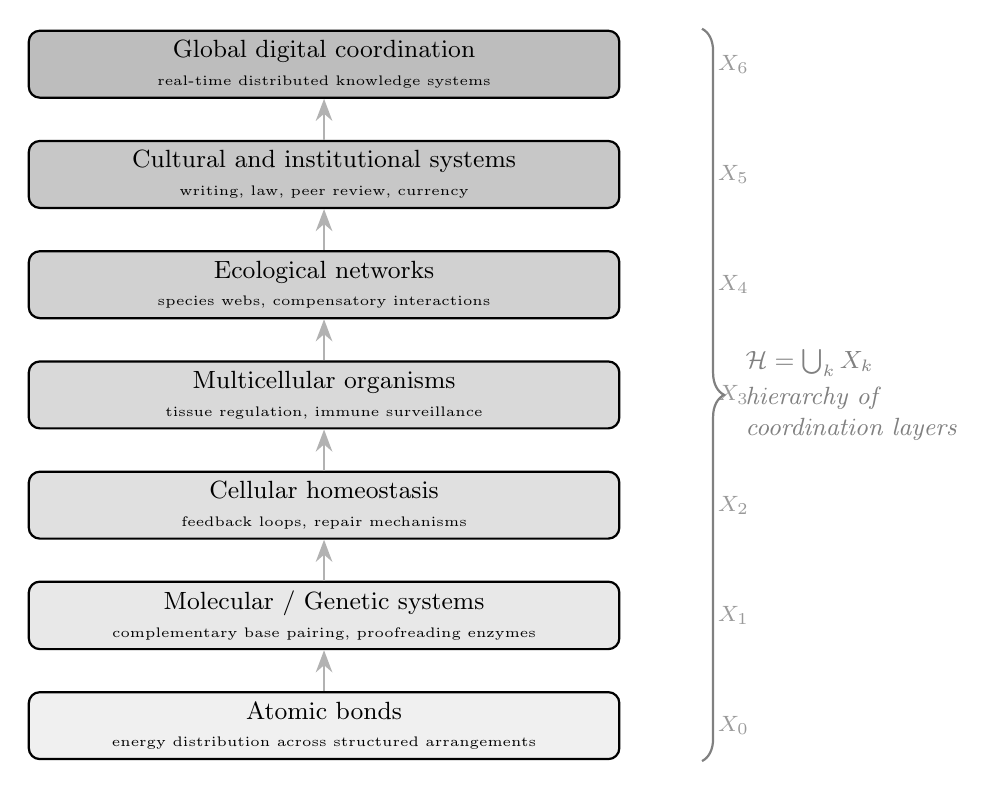
\begin{tikzpicture}[
  level/.style={rectangle, rounded corners=4pt, draw=black, thick,
                minimum width=7.5cm, minimum height=0.85cm,
                font=\small, align=center},
  arrow/.style={-{Stealth[length=8pt]}, thick, gray!60},
  annot/.style={font=\footnotesize\itshape, text=gray!80, align=left}
]

\node[level, fill=gray!12] (L0) at (0,0)    {Atomic bonds\\[-1pt]{\tiny energy distribution across structured arrangements}};
\node[level, fill=gray!18] (L1) at (0,1.4)  {Molecular / Genetic systems\\[-1pt]{\tiny complementary base pairing, proofreading enzymes}};
\node[level, fill=gray!24] (L2) at (0,2.8)  {Cellular homeostasis\\[-1pt]{\tiny feedback loops, repair mechanisms}};
\node[level, fill=gray!30] (L3) at (0,4.2)  {Multicellular organisms\\[-1pt]{\tiny tissue regulation, immune surveillance}};
\node[level, fill=gray!36] (L4) at (0,5.6)  {Ecological networks\\[-1pt]{\tiny species webs, compensatory interactions}};
\node[level, fill=gray!44] (L5) at (0,7.0)  {Cultural and institutional systems\\[-1pt]{\tiny writing, law, peer review, currency}};
\node[level, fill=gray!52] (L6) at (0,8.4)  {Global digital coordination\\[-1pt]{\tiny real-time distributed knowledge systems}};

\foreach \a/\b in {L0/L1, L1/L2, L2/L3, L3/L4, L4/L5, L5/L6}
  \draw[arrow] (\a.north) -- (\b.south);

\node[annot] at (5.2, 0)   {$X_0$};
\node[annot] at (5.2, 1.4) {$X_1$};
\node[annot] at (5.2, 2.8) {$X_2$};
\node[annot] at (5.2, 4.2) {$X_3$};
\node[annot] at (5.2, 5.6) {$X_4$};
\node[annot] at (5.2, 7.0) {$X_5$};
\node[annot] at (5.2, 8.4) {$X_6$};

\draw[decorate, decoration={brace, amplitude=8pt, mirror}, thick, gray]
  (4.8, -0.45) -- (4.8, 8.85)
  node[midway, right=12pt, font=\small\itshape, align=left] {$\mathcal{H} = \bigcup_k X_k$\\[2pt]hierarchy of\\coordination layers};

\end{tikzpicture}
\caption{Hierarchical error-correcting layers across biological and social scales. Each level $X_k$ aggregates components from $X_{k-1}$ through a coordination operator $F_{k-1}: X_{k-1}^n \to X_k$ that introduces redundancy, feedback, and constraint structures increasing robustness against noise. Civilization occupies the uppermost levels currently instantiated.}
\label{fig:hierarchy}
\end{figure}

At the atomic level, stable molecules arise because atomic bonds distribute energy across structured arrangements that resist perturbation. At the molecular level, genetic systems encode biological information using redundant mechanisms such as complementary base pairing and proofreading enzymes that detect and repair transcription errors.

Cells themselves are networks of feedback loops that maintain homeostasis despite constant environmental fluctuations. Multicellular organisms extend this principle further: tissues and organs coordinate through regulatory systems that detect deviations from stable states and restore equilibrium. Ecosystems exhibit similar dynamics. Species interact through webs of mutual dependence that stabilize environmental conditions over long periods of time.

Human civilization can be interpreted within this same framework. Large societies create distributed systems for storing, transmitting, and correcting information across generations. Written language preserves knowledge beyond the lifespan of individuals. Scientific institutions refine and verify claims through collective scrutiny. Legal systems encode shared expectations that regulate social behavior.

In this sense, civilization functions as a large-scale error-correcting structure. Seen from this perspective, the emergence of civilization is not a deviation from the principles that govern biological evolution. It is a continuation of them.

\subsection{Hierarchical Error-Correcting Layers}

The recurrence of cooperative structures across biological and social scales can be described more formally as a hierarchy of error-correcting layers. Each layer aggregates lower-level units into a larger system that stabilizes information and behavior in the presence of noise.

Let a system at scale $k$ consist of a collection of interacting components
\[
X_k = \{x_1, x_2, \dots, x_n\}.
\]
The collective dynamics of these components produce a higher-order structure
\[
X_{k+1} = F_k(X_k),
\]
where $F_k$ represents the coordination mechanism that integrates the lower-level units into a coherent whole.

Crucially, the function $F_k$ does more than simply aggregate components. It introduces redundancy, feedback, and constraint structures that allow the higher-level system to detect and correct deviations produced by noise in the underlying processes. In this sense, the transition from $X_k$ to $X_{k+1}$ functions analogously to an error-correcting code in information theory: information that would be unstable at the lower level becomes robust once distributed across the higher-level structure.

The emergence of civilization can therefore be interpreted as the formation of a new layer in the hierarchy of error-correcting organization. Individual humans, each subject to cognitive limitations and environmental uncertainty, become components of larger systems that preserve and refine information collectively. From this perspective, complexity grows not through the elimination of noise but through the construction of structures capable of managing it.

\section{Phase Transitions in Coordination Regimes}
\label{sec:phase}

The language of collapse implies catastrophic and irreversible discontinuity. The language of phase transition, by contrast, designates a structural reorganization in which qualitative behavior changes as system parameters cross critical thresholds. The distinction is not merely semantic: it has precise mathematical content within the theory of dynamical systems, and it determines whether the appropriate response to civilizational disruption is alarm or adaptation.

\subsection{Bifurcation Theory and Institutional Dynamics}

Consider a parameterized family of dynamical systems
\[
\dot{x} = f_\mu(x), \qquad x \in \mathbb{R}^n, \quad \mu \in \mathbb{R},
\]
where $\mu$ represents a control parameter encoding the state of the technological or informational infrastructure supporting social coordination---communication bandwidth, energy surplus, institutional redundancy, or analogous quantities.

A bifurcation occurs at a critical value $\mu_c$ when the qualitative structure of the phase portrait changes: equilibria are created or destroyed, their stability changes, or limit cycles appear. The most elementary such transition is the saddle-node bifurcation, in which two equilibria coalesce and annihilate, leaving the system with a single stable state whose basin of attraction encompasses the region previously governed by the destroyed equilibrium. More relevant to institutional dynamics is the pitchfork bifurcation, depicted in Figure~\ref{fig:bifurcation}.

\begin{figure}[ht]
\centering
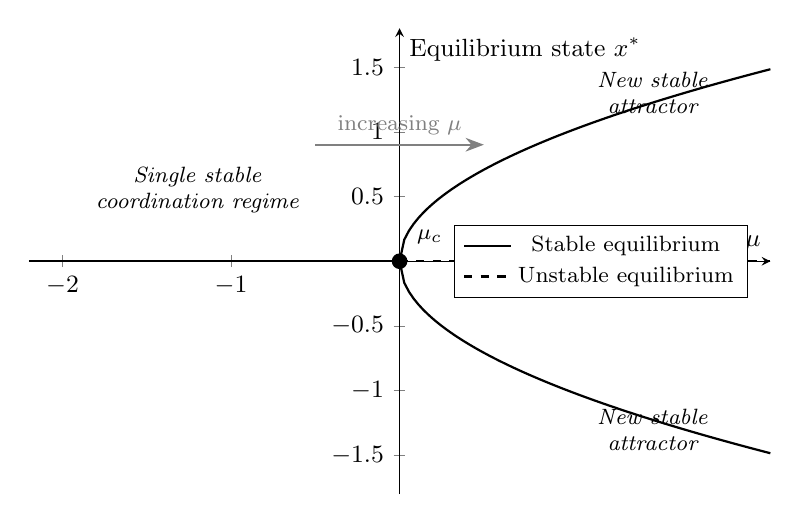
\begin{tikzpicture}
\begin{axis}[
  width=11cm, height=7.5cm,
  xlabel={Control parameter $\mu$},
  ylabel={Equilibrium state $x^*$},
  xmin=-2.2, xmax=2.2,
  ymin=-1.8, ymax=1.8,
  axis lines=center,
  xtick={-2,-1,0,1,2},
  ytick={-1.5,-1,-0.5,0,0.5,1,1.5},
  tick label style={font=\small},
  label style={font=\small},
  legend style={at={(0.97,0.5)}, anchor=east, font=\footnotesize},
  clip=false,
]

% Stable branch: x=0 for mu < 0
\addplot[thick, black, domain=-2.2:0, samples=2]
  coordinates {(-2.2,0) (0,0)};
\addlegendentry{Stable equilibrium}

% Unstable branch: x=0 for mu > 0
\addplot[thick, black, dashed, domain=0:2.2, samples=2]
  coordinates {(0,0) (2.2,0)};
\addlegendentry{Unstable equilibrium}

% Upper stable branch for mu > 0: x = sqrt(mu)
\addplot[thick, black, domain=0:2.2, samples=80]
  {sqrt(x)};

% Lower stable branch for mu > 0: x = -sqrt(mu)
\addplot[thick, black, domain=0:2.2, samples=80]
  {-sqrt(x)};

% Bifurcation point annotation
\node[circle, fill=black, inner sep=2pt] at (axis cs:0,0) {};
\node[font=\footnotesize, above right=4pt] at (axis cs:0,0) {$\mu_c$};

% Region annotations
\node[font=\footnotesize\itshape, align=center] at (axis cs:-1.2, 0.55)
  {Single stable\\coordination regime};
\node[font=\footnotesize\itshape, align=center] at (axis cs:1.5, 1.3)
  {New stable\\attractor};
\node[font=\footnotesize\itshape, align=center] at (axis cs:1.5,-1.3)
  {New stable\\attractor};
\node[font=\footnotesize\itshape, align=center] at (axis cs:1.0, 0.18)
  {\textit{(unstable)}};

% Arrow indicating transition direction
\draw[-{Stealth}, gray, thick] (axis cs:-0.5,0.9) -- (axis cs:0.5,0.9)
  node[midway, above, font=\footnotesize] {increasing $\mu$};

\end{axis}
\end{tikzpicture}
\caption{Supercritical pitchfork bifurcation as a model of institutional phase transition. For $\mu < \mu_c$ a unique stable coordination equilibrium exists. At the critical parameter value $\mu_c$---corresponding, for instance, to the introduction of a transformative communication technology---the single equilibrium loses stability, and two new stable attractors emerge. The period of institutional turbulence observed during technological transitions corresponds to the neighborhood of $\mu_c$, during which the system reorganizes toward a new attractor rather than collapsing. This pattern generalizes to higher-dimensional bifurcations appropriate for multi-regime coordination.}
\label{fig:bifurcation}
\end{figure}

In the context of civilizational dynamics, the control parameter $\mu$ may be interpreted as a composite index of technological capacity. As this parameter increases through a critical threshold, the previously stable institutional equilibrium loses its stability and the system reorganizes around new attractors. The period of maximal observed turbulence---polarization, institutional dysfunction, erosion of epistemic commons---corresponds to the neighborhood of $\mu_c$, where the system has departed from the old attractor but has not yet converged to the new ones.

\subsection{Catastrophe vs. Phase Transition}

The conceptual distinction between collapse and phase transition can be formalized through catastrophe theory. A fold catastrophe corresponds to the sudden disappearance of a stable equilibrium with no replacement: the system is thrown into open dynamics with no nearby attractor. A phase transition, by contrast, preserves the density of attractors while changing their location and basin structure.

The empirical evidence from historical transitions---the agricultural revolution, the emergence of literacy, the industrial revolution---consistently suggests the phase transition pattern rather than the fold catastrophe. In each case, periods of marked instability were followed by the consolidation of new institutional forms operating in qualitatively different parameter regimes. The relevant question for the present moment is therefore not whether equilibrium will be restored but which of the emergent attractors human societies will converge toward and how that convergence can be guided.

\subsection{Hysteresis and Path Dependence}

Phase transitions in coordination regimes exhibit hysteresis: the path taken through parameter space determines which attractor is approached, and the system cannot simply be returned to its prior state by reversing the parameter change. This has important normative implications. There is no path back to pre-industrial coordination structures, nor is one desirable: the informational and material complexity that characterizes contemporary life cannot be sustained by the coordination mechanisms of an earlier era. The appropriate response to phase transition is forward design of institutional forms suited to the new parameter regime, not retrospective idealization of prior states.

\section{Scientific Institutions as Knowledge Stabilizers}

If civilization functions as a large-scale coordination system, its most distinctive institutions can be understood as mechanisms for stabilizing knowledge across time. Human cognition is inherently limited and error-prone. Individuals forget, misinterpret, and repeat mistakes. Without external structures for preserving and correcting information, complex knowledge would dissipate rapidly---a phenomenon that can be quantified: if the probability of faithful transmission of any given cognitive item is $p < 1$, then after $n$ generations the probability of intact preservation is $p^n \to 0$. Institutional error correction breaks this exponential decay by distributing information redundantly and introducing active verification.

Scientific institutions evolved as a response to this problem. Written records allow observations to persist beyond the lifespan of the observer. Replication procedures allow independent groups to verify results under different conditions. Peer review introduces distributed scrutiny, increasing the likelihood that errors will be detected and corrected before claims become widely accepted.

These practices resemble error-correcting processes in information systems. Rather than relying on the reliability of any single observer, scientific communities distribute the task of verification across many participants. Knowledge becomes robust not because individuals are infallible but because institutional structures allow mistakes to be identified and revised. Over time these mechanisms allow societies to accumulate reliable knowledge across generations. This cumulative process represents one of civilization's most powerful coordination achievements, and the persistence of such systems further undermines the claim that civilization is inherently self-destructive.

\section{The Myth of the Agricultural Trap}

A central claim in many critiques of civilization is that the transition from nomadic hunter--gatherer societies to agricultural settlement constituted a historical mistake. According to this view, early humans exchanged mobility and egalitarian social structures for sedentary life, territorial competition, and hierarchical institutions. Agriculture is therefore portrayed as a trap: once adopted, it locked humanity into systems of labor, property, and inequality that could no longer be escaped.

This interpretation captures an important historical reality. The agricultural transition did transform human societies in profound ways. Cultivation tethered populations to specific territories, encouraged the accumulation of surplus resources, and made it possible for some individuals to specialize in roles other than subsistence food gathering. These changes created the conditions under which political hierarchies and economic inequalities could emerge.

However, describing agriculture as a ``trap'' misunderstands both the nature of the transition and its long-term consequences, and conflates a change in coordination parameter regime with a moral fall. Agriculture did not merely introduce hierarchy; it also dramatically expanded the scale and complexity of human coordination. The production of reliable food surpluses enabled permanent settlements, which in turn made possible the emergence of cities, long-distance trade networks, and specialized intellectual labor. Systems of writing, mathematics, law, and scientific observation all developed within agricultural civilizations.

Archaeological and anthropological evidence also complicates the romantic image of pre-agricultural life. Hunter--gatherer societies were often socially cohesive and flexible, but they were also constrained by strict ecological limits. Population densities remained low because the carrying capacity of foraging environments could support only small groups. Life expectancy was short, infant mortality high, and injuries or infections that are easily treatable today were frequently fatal. The comparison is not between freedom and unfreedom but between two different parameter regimes of coordination, each with its characteristic tradeoffs.

From the phase-transition perspective developed in the preceding section, the agricultural transition is precisely a bifurcation event: a new coordination technology shifted the effective control parameter past a threshold, destabilizing existing social equilibria and generating new attractors characterized by hierarchy, surplus, and specialization. The turbulence of the transition was real. But the transition itself was not a trap. It was the formation of a new coordination layer in the hierarchy.

\section{The Expanding Radius of Human Concern}

A second common argument holds that modern civilization produces unprecedented loneliness and alienation. According to this view, humans evolved for life in small tribes of a few dozen individuals, and modern cities replace those intimate social environments with vast populations of strangers. Physical proximity increases while emotional connection diminishes.

This interpretation captures an important psychological tension, but it also overlooks a profound transformation in the scale of human social imagination. Rather than contracting, the circle of human concern has expanded dramatically over the course of civilization. The moral expectations placed upon individuals in modern societies increasingly extend far beyond the boundaries of tribe, kinship, or immediate locality.

In earlier forms of social organization, moral obligations were largely restricted to a small in-group. Modern communication networks and global institutions have begun to alter these patterns by enabling sustained interaction across enormous distances. The result is not simply the replacement of tribal bonds with anonymity. It is the emergence of connections that span what might be called \emph{geozotic distance}: the combined separation produced by geography, culture, language, and ideology. Individuals are now able to form intellectual, cultural, and cooperative relationships with others embedded in entirely different social environments. The metric formalization of geozotic distance is developed in Appendix~\ref{app:geozotic}.

Digital communication networks illustrate this transformation clearly. Communities of practice, research collaboration, artistic production, and political dialogue increasingly operate at global scales. At the same time, the scope of moral consideration has expanded beyond humanity itself. Environmental ethics, animal welfare movements, and ecological awareness reflect an emerging recognition that human societies exist within broader living systems.

These developments suggest that what appears to be the dissolution of traditional social structures may instead represent the expansion of human relational capacity. The challenge is not that humans are incapable of connection in large societies, but that our institutions and cultural practices are still adapting to a world in which the potential scale of connection has grown far beyond anything previously experienced.

\section{Civilization as a Coordination Engine}

The preceding discussions suggest that critiques of civilization often begin from a mistaken premise. Civilization is frequently treated as a moral condition or psychological environment that can be evaluated in terms of authenticity, alienation, or spiritual health. Yet historically civilization has functioned primarily as something else: a coordination technology. Its moral quality is not intrinsic but is a function of how its mechanisms are designed and for what purposes they are deployed.

Human societies must solve a fundamental problem. Large numbers of individuals must synchronize their actions across time and space in order to produce food, construct infrastructure, transmit knowledge, and maintain social order. The mechanisms that make such synchronization possible are what constitute civilization.

Early hunter--gatherer bands coordinated through kinship structures, oral traditions, and immediate face-to-face interaction. The transition to agriculture introduced new coordination tools, including territorial governance, stored surplus, written records, and administrative institutions. Over time additional coordination mechanisms emerged: systems of writing, monetary systems, legal institutions, scientific methods. Industrialization introduced yet another layer: railways, telegraphs, electrical grids, and global shipping networks synchronized production and distribution across continents. Today digital networks are transforming coordination once again.

Seen from this perspective, civilization is not a static entity but a continuously evolving architecture of coordination. Each major technological shift alters the mechanisms through which large populations organize themselves. When these mechanisms change rapidly, existing institutions often struggle to adapt. Periods of institutional instability may therefore reflect transitions in coordination architecture rather than the failure of civilization itself.

Understanding civilization as a coordination engine clarifies many contemporary tensions. Systems designed for earlier technological environments may no longer function efficiently within new informational infrastructures. Economic institutions built for industrial production must adapt to digital knowledge economies. Political institutions developed for slower communication environments must operate within instantaneous global media ecosystems. These mismatches generate the impression that the entire civilizational system is failing. In reality, they indicate that the coordination mechanisms supporting civilization are being reorganized.

\section{Mistaking Transition for Collapse}

Once civilization is understood as an evolving coordination system, a pattern becomes visible across history. Periods in which the underlying infrastructure of coordination changes rapidly are frequently experienced by contemporaries as moments of profound instability. Institutions designed for one technological environment often function poorly when the informational and material substrate supporting them begins to shift. The resulting turbulence can easily be interpreted as evidence that the entire social order is failing.

Historical precedents illustrate this dynamic clearly. The transition from foraging to agriculture, as argued above, precipitated a bifurcation in social organization. A similar pattern emerged during the industrial revolution. The introduction of mechanized production, fossil energy, and rapid transportation disrupted centuries-old economic and social arrangements. Observers living through the early phases of industrialization frequently described their societies as morally and socially disintegrating.

Yet with time new institutional frameworks emerged that stabilized these transformations. Public education systems, labor law, democratic governance structures, and modern regulatory institutions gradually developed in response to the demands of industrial coordination. What initially appeared as civilizational disintegration eventually produced a new equilibrium adapted to the technological conditions of the era.

The contemporary world may be experiencing a comparable transformation. Digital communication networks, computational infrastructure, and global information flows have altered the speed and scale at which coordination occurs. Institutions built during the industrial period often struggle to function effectively within this new informational environment. When such mismatches occur, institutions can appear dysfunctional or incoherent. These symptoms can resemble civilizational decline when viewed in isolation. However, they may also represent the early stages of a structural reconfiguration.

The crucial distinction is therefore between collapse and transition. Collapse implies the irreversible breakdown of social complexity and the loss of coordination capacity. Transition, by contrast, involves the reorganization of coordination mechanisms in response to new technological and informational conditions. The visible instability of the present moment does not necessarily imply the disappearance of civilization; it may indicate that civilization is undergoing another phase in its long process of institutional evolution.

\section{Civilization Is Not a Disease}

Another common rhetorical strategy in critiques of modern society is to describe civilization as a kind of pathology. Civilization is compared to an illness, an addiction, or a slow-moving infection that humanity has contracted and cannot escape.

The metaphor is rhetorically vivid but conceptually unstable. A disease, in the strict sense, is a condition that organisms attempt to eliminate or recover from. Civilization does not exhibit these characteristics. People do not behave toward civilization as they behave toward disease. On the contrary, they continuously reproduce, maintain, and expand the institutions that constitute it. Even individuals who criticize modern society typically do so using the very tools that civilization provides: writing, digital communication networks, global distribution platforms, and technological infrastructure. The critique of civilization is therefore itself a civilizational activity.

This observation reveals the limits of the pathological metaphor. A condition that populations actively maintain, improve, and defend cannot be meaningfully described as a disease. It may involve tradeoffs, tensions, and unintended consequences, but it functions more accurately as an adaptive system. Civilization persists not because humanity is helplessly addicted to it, but because it provides coordination capacities that no previous form of social organization could sustain.

\section{The Future of Human Coordination}

If civilization is understood as a coordination engine rather than a pathological condition, the central question of the present era changes significantly. The problem is no longer how to escape civilization, but how to guide the next stage in the evolution of its coordination mechanisms.

Human societies have repeatedly expanded the scale at which cooperation is possible. The digital era is expanding that scale once again. Communication networks now allow individuals separated by thousands of kilometers to collaborate in real time. Knowledge repositories accumulate contributions from millions of participants. Scientific, artistic, and technical communities operate across national and cultural boundaries.

This expansion also reshapes the moral imagination of societies. Such developments do not eliminate the tensions associated with large-scale societies. Coordination at planetary scale introduces new forms of complexity and conflict that earlier institutions were not designed to manage. Political systems, economic frameworks, and cultural norms must adapt to conditions in which information flows rapidly and social interactions extend across enormous geozotic distances.

Periods of institutional experimentation and instability are therefore likely to accompany this transformation. Yet instability should not be confused with civilizational failure. The future of civilization will depend on the capacity of human societies to design institutions that align with the technological and informational environments they inhabit. Civilization has never been a finished project. It is a dynamic process through which humans continually invent new ways of living together.

\section{Theory-Ladenness and the Illusion of the ``Gish Gallop''}

Debates about civilization frequently become entangled in a rhetorical accusation known as the ``Gish gallop.'' The term refers to a debate tactic in which a speaker rapidly presents a large number of arguments or claims in succession, overwhelming an opponent's ability to respond to each one individually.

However, the accusation of a Gish gallop can sometimes obscure a deeper epistemological phenomenon known as \emph{theory-ladenness}. In the philosophy of science, observations are not interpreted in isolation but through conceptual frameworks that determine what counts as evidence and how different facts relate to one another \cite{hanson1958,kuhn1962}. Perception itself is shaped by theoretical commitments.

When two interlocutors operate within different conceptual frameworks, a series of observations that form a coherent pattern within one framework may appear as an incoherent list of unrelated claims within another. This dynamic is particularly visible in discussions of complex systems such as civilization. Evidence drawn from biology, ecology, information theory, and social organization may converge toward a unified interpretation when viewed through a coordination-based framework. Yet to an observer who interprets these domains separately, the same collection of observations may appear as a scattered set of arguments delivered too quickly to evaluate.

In such cases the difficulty does not arise from the quantity of claims alone, but from the absence of a shared theoretical structure capable of organizing them. Recognizing the role of theory-ladenness clarifies why debates about civilization often feel unproductive. Participants are not merely disagreeing about individual facts; they are interpreting those facts through fundamentally different models of how complex systems evolve. Until those underlying models are made explicit, the conversation risks oscillating between accusations of rhetorical manipulation and frustration at the inability to communicate structural insights.

\subsection{Competing Interpretive Frameworks}

The persistence of disagreement in discussions of civilizational decline can therefore be understood as a conflict between interpretive frameworks rather than a dispute over isolated facts. Two broad explanatory models tend to organize the available evidence in different ways.

Within the collapse narrative, observations about inequality, ecological stress, technological disruption, and psychological distress are interpreted as symptoms of systemic pathology. Within a coordination-based framework, the same observations can be interpreted as indicators of phase transition in coordination architecture.

Because these frameworks structure the interpretation of evidence differently, the same body of observations can support opposite conclusions. Progress therefore requires examining the underlying models through which evidence is organized. The formal frameworks developed in the appendices---dynamical systems theory, coding theory, sheaf theory, category theory---provide the theoretical infrastructure through which this examination can be conducted with precision.

\section{Civilization as Planetary Information Processing}

Taken together, these observations suggest that civilization may be understood as the biosphere's first large-scale information processing system. Biological evolution has always depended on the storage, transmission, and correction of information. Human civilization extends these processes into a new domain: cultural practices, written language, scientific institutions, and technological infrastructures collectively function as mechanisms for storing and refining information about the world at speeds and scales unavailable to purely biological systems.

What distinguishes civilization from earlier biological systems is the scale and speed at which this informational coordination occurs. In this sense civilization represents a continuation of evolutionary processes rather than a deviation from them. The emergence of such a system does not eliminate instability or conflict. Complex information-processing structures inevitably encounter periods of turbulence as they adapt to new conditions. Yet the presence of distributed mechanisms for learning and correction suggests that civilization possesses powerful tools for responding to these challenges.

Rather than marking the exhaustion of human development, civilization may represent the beginning of a new phase in which the biosphere acquires the capacity to understand and reshape its own trajectory.

\section{Conclusion}

The narrative of civilizational collapse often emerges during moments of rapid transformation. When familiar institutions begin to strain under new technological and social conditions, the resulting turbulence can create the impression that the entire project of civilization has reached its limits. Yet history suggests a different interpretation, one that the formal frameworks developed here allow to be stated with precision: periods of disruption frequently correspond to bifurcations in the dynamical parameter space of coordination, in which old institutional equilibria lose stability and new attractors emerge.

Agriculture did not end human freedom; it expanded the scale of cooperation beyond the limits of small bands. Industrialization did not destroy society; it reorganized production and governance around new sources of energy and infrastructure. The contemporary world appears to be undergoing a comparable transition, driven by the emergence of digital coordination technologies.

What appears to some observers as civilizational decline is more plausibly interpreted as the approach to a bifurcation point: the existing institutional equilibria, designed for an earlier coordination regime, are losing stability, and the system is reorganizing toward new attractors whose character is not yet determined. The visible instability of this reorganization is not evidence of systemic failure. It is evidence of systemic change.

Civilization is not a completed structure nor an irreversible mistake. It is an ongoing experiment in large-scale cooperation, and a mathematically non-trivial one: its persistence requires the continual construction and maintenance of error-correcting structures at multiple scales, the ongoing negotiation of phase transitions in coordination architecture, and the design of institutions capable of preserving human dignity and ecological stability within parameter regimes of unprecedented complexity. These are engineering problems as much as moral ones, and addressing them requires the kind of formal precision that this essay has sought, at least in preliminary form, to bring to bear.

\newpage
\section*{Appendices}

\appendix

\section{Multiscale Coordination Systems}

Many complex systems are organized through nested layers of coordination in which collections of interacting components at one scale give rise to stable structures at higher scales. This appendix formalizes such systems as a hierarchy of coordination operators acting on sets of interacting agents.

\subsection{Base Level Components}

Let
\[
X_0 = \{x_1, x_2, \dots , x_n\}
\]
denote the set of elementary components of the system. These components may represent agents, cells, organisms, or other interacting units depending on the level of description.

\subsection{Coordination Operators}

Higher levels of organization emerge through coordination maps
\[
F_k : X_k^n \rightarrow X_{k+1},
\]
which transform collections of interacting elements at level $k$ into coordinated structures at level $k+1$.

The resulting hierarchy is therefore defined recursively as
\[
X_{k+1} = F_k(X_k).
\]

Each level aggregates the elements of the previous level into higher-order structures.

\subsection{Nested Organizational Structure}

The hierarchy of coordinated systems forms a nested sequence
\[
X_0 \subset X_1 \subset X_2 \subset \dots \subset X_k .
\]

The full hierarchy of coordinated structures can therefore be represented as the union
\[
\mathcal{H} = \bigcup_{k=0}^{\infty} X_k .
\]

When the sequence converges in an appropriate topology, we may define the asymptotic coordination structure
\[
\lim_{k \to \infty} X_k .
\]

\subsection{System Observables}

Each coordination level is associated with an observable functional
\[
\Phi_k : X_k \rightarrow \mathbb{R},
\]
which measures a macroscopic property of the system at that level. Examples include energy, information content, coordination efficiency, or entropy production.

\subsection{Dynamical Evolution}

The state of each coordination layer evolves according to a dynamical system
\[
\frac{dX_k}{dt} = G_k(X_k),
\]
where
\[
G_k : X_k \rightarrow T X_k
\]
is a vector field on the state space $X_k$, and $T X_k$ denotes the tangent bundle of $X_k$.

\subsection{Projection Operators}

To maintain coherence between levels of the hierarchy, we introduce projection maps
\[
\pi_k : X_{k+1} \rightarrow X_k ,
\]
which recover the lower-level representation of a higher-level coordinated structure.

Consistency between levels requires the compatibility condition
\[
\pi_k \circ F_k = \mathrm{id}_{X_k},
\]
ensuring that projecting a coordinated structure back to the lower level reproduces the original configuration.

\subsection{Stability of Multiscale Coordination}

\begin{theorem}[Hierarchical Coordination Stability]
Let $\{X_k\}_{k=0}^{\infty}$ be a hierarchy of coordination spaces with coordination operators
$F_k : X_k^n \rightarrow X_{k+1}$
and projection maps
$\pi_k : X_{k+1} \rightarrow X_k$
satisfying $\pi_k \circ F_k = \mathrm{id}_{X_k}$.
Assume that each level evolves under $\dot{X}_k = G_k(X_k)$ with $G_k$ locally Lipschitz.
If there exists a family of Lyapunov functionals $\Phi_k : X_k \to \mathbb{R}$ such that
$\tfrac{d}{dt}\Phi_k(X_k) \le 0$ for all $k$, then the multiscale coordination hierarchy admits a stable invariant manifold
$\mathcal{M} \subset \mathcal{H}$ such that $\lim_{t \to \infty} X_k(t) \in \mathcal{M}$.
\end{theorem}

\begin{proof}
The compatibility condition ensures that the hierarchy forms a consistent inverse system. Lipschitz regularity of $G_k$ guarantees existence and uniqueness of solutions on finite intervals. The Lyapunov condition implies that trajectories remain within sublevel sets of $\Phi_k$, which are forward-invariant. The nested structure $X_0 \subset X_1 \subset \cdots$ allows us to define
\[
\mathcal{M} = \bigcap_{k=0}^{\infty} \{ X_k \mid \Phi_k(X_k) \le c_k \}.
\]
By LaSalle's invariance principle, trajectories converge to $\mathcal{M}$ as $t \to \infty$.
\end{proof}

\section{Error-Correcting Coordination}

\subsection{Message Space and Encoding}

Let $M = \{m_1, \dots, m_n\}$ be a finite message space. An encoding
\[
C : M \rightarrow \Sigma^n
\]
into a code of block length $n$ over alphabet $\Sigma$ introduces redundancy enabling recovery under noise.

\subsection{Distance Structure and Error Correction}

For $x,y \in \Sigma^n$ define $d(x,y) = \sum_i |x_i - y_i|$. The minimum code distance is $d_{\min} = \min_{x \neq y} d(x,y)$, yielding correction radius
\[
t = \left\lfloor \tfrac{d_{\min}-1}{2} \right\rfloor.
\]

\begin{theorem}[Redundancy--Stability]
Let $C : M \to \Sigma^n$ be an injective encoding with minimum distance $d_{\min}$. If $|e| \le t$, there exists a decoding map $R : \Sigma^n \to M$ such that $R(C(m)+e)=m$ for every $m \in M$. Moreover, if $d_{\min}^{(2)} > d_{\min}^{(1)}$ for two encodings, then their correction radii satisfy $\lfloor \tfrac{d_{\min}^{(2)}-1}{2} \rfloor \ge \lfloor \tfrac{d_{\min}^{(1)}-1}{2} \rfloor$.
\end{theorem}

\begin{proof}
Since the codewords have minimum pairwise distance $d_{\min}$, the closed metric balls of radius $t$ around distinct codewords are disjoint. Indeed, suppose $d(z,x) \le t$ and $d(z,y) \le t$ for distinct $x,y \in C(M)$; then $d(x,y) \le 2t < d_{\min}$, a contradiction. Nearest-neighbor decoding on the disjoint balls yields the required $R$. Monotonicity of $d \mapsto \lfloor (d-1)/2 \rfloor$ gives the second statement.
\end{proof}

\begin{corollary}
Increasing representational redundancy so that $d_{\min}$ increases cannot decrease the system's tolerance to bounded perturbations.
\end{corollary}

\section{Cooperative Evolutionary Dynamics}

Let $x = (x_1,\dots,x_n) \in \Delta^n$ denote the population distribution, where $\Delta^n = \{x \ge 0 \mid \sum_i x_i = 1\}$. With payoff matrix $A$, fitness $f_i = (Ax)_i$, and mean fitness $\phi = x^T Ax$, the replicator equation is
\[
\dot{x}_i = x_i(f_i - \phi).
\]
This flow preserves the simplex since $\sum_i \dot{x}_i = \phi - \phi = 0$. An equilibrium $x^*$ satisfies $(Ax^*)_i = (x^*)^T Ax^*$ whenever $x_i^* > 0$.

\section{Information Accumulation}

Shannon entropy $H(X) = -\sum p(x)\log p(x)$ and mutual information $I(X;Y) = H(X) - H(X|Y)$ quantify uncertainty and structured dependence. Kolmogorov complexity $K(x) = \min_{p: U(p)=x} |p|$ measures minimal descriptive length. The iterative accumulation law
\[
I_{t+1} = I_t + \Delta I_t, \qquad \Delta I_t = f(E_t, S_t),
\]
expresses the principle that complex systems persist by incorporating new information into existing organizational memory.

\section{Hierarchical Stability}

\subsection{Gradient Flow Dynamics}

Suppose aggregate state $S_k \in \mathbb{R}^m$ evolves under gradient flow $\dot{S}_k = -\nabla V(S_k)$ with quadratic potential $V(S_k) = \tfrac{1}{2} S_k^T A S_k$.

\begin{theorem}[Lyapunov Stability]
If $A \in \mathbb{R}^{m \times m}$ is symmetric positive definite, then $S_k^* = 0$ is globally asymptotically stable.
\end{theorem}

\begin{proof}
$V$ is positive definite with $\nabla V = AS_k$, so the dynamics are $\dot{S}_k = -AS_k$. Along trajectories:
\[
\tfrac{d}{dt}V = (AS_k)^T(-AS_k) = -S_k^T A^2 S_k < 0 \quad (S_k \neq 0),
\]
since $A^2$ is positive definite. Radial unboundedness of $V$ gives global convergence to $0$.
\end{proof}

\begin{corollary}
If each hierarchical update $S_{k+1} = F(S_k)$ maps asymptotically stable equilibria to asymptotically stable equilibria, the hierarchy $\{S_k\}$ defines a stability-preserving multiscale coordination system.
\end{corollary}

\section{Categorical Coordination Structures}

\subsection{Categories and Functors}

Let $\mathcal{C}_0, \mathcal{C}_1, \dots, \mathcal{C}_k$ be a sequence of categories, each with objects, morphisms, associative composition, and identities. Coordination transitions between levels are represented by functors $F_k : \mathcal{C}_k \to \mathcal{C}_{k+1}$ satisfying
\[
F_k(f \circ g) = F_k(f) \circ F_k(g), \qquad F_k(\mathrm{id}_x) = \mathrm{id}_{F_k(x)}.
\]

The sequence $\mathcal{C}_0 \to \mathcal{C}_1 \to \cdots$ forms a directed system with direct limit $\mathcal{C}_\infty = \varinjlim \mathcal{C}_k$.

\begin{theorem}[Functorial Preservation]
Functors preserve commutative diagrams: if $h = g \circ f$ in $\mathcal{C}_k$, then $F_k(h) = F_k(g) \circ F_k(f)$ in $\mathcal{C}_{k+1}$.
\end{theorem}

\begin{theorem}[Adjunction and Aggregation]
Let $F \dashv G$ with $F : \mathcal{C} \to \mathcal{D}$ and $G : \mathcal{D} \to \mathcal{C}$. Then $\Hom_\mathcal{D}(F(X),Y) \cong \Hom_\mathcal{C}(X,G(Y))$ naturally. Every higher-level coordination map $F(X) \to Y$ corresponds to a lower-level map $X \to G(Y)$.
\end{theorem}

\section{Graph Coordination Dynamics}

Let $G=(V,E)$ with Laplacian $L = D - A$. The consensus system $\dot{x} = -Lx$ has solution $x(t) = e^{-Lt}x_0$.

\begin{theorem}[Exponential Consensus]
For a connected undirected graph with algebraic connectivity $\lambda_2 > 0$:
\[
\|x(t) - \bar{x}\mathbf{1}\| \le e^{-\lambda_2 t}\|x_0 - \bar{x}\mathbf{1}\|,
\quad \bar{x} = \tfrac{1}{n}\mathbf{1}^T x_0.
\]
\end{theorem}

\begin{proof}
Decompose $x_0 = \sum_i \alpha_i v_i$ in the eigenbasis of $L$. The zero-eigenspace contribution is $\bar{x}\mathbf{1}$, so $x(t) - \bar{x}\mathbf{1} = \sum_{i \ge 2} \alpha_i e^{-\lambda_i t}v_i$. Using $\lambda_i \ge \lambda_2$ for $i \ge 2$ and orthonormality gives the bound.
\end{proof}

Figure~\ref{fig:consensus} illustrates the convergence of four agents to the mean state under consensus dynamics on a connected graph.

\begin{figure}[ht]
\centering
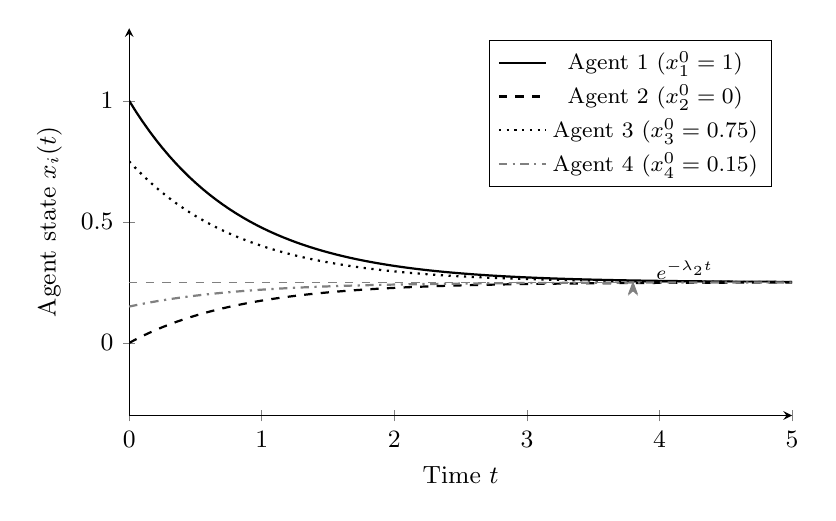
\begin{tikzpicture}
\begin{axis}[
  width=10cm, height=6.5cm,
  xlabel={Time $t$},
  ylabel={Agent state $x_i(t)$},
  xmin=0, xmax=5,
  ymin=-0.3, ymax=1.3,
  axis lines=left,
  legend pos=north east,
  legend style={font=\footnotesize},
  tick label style={font=\small},
  label style={font=\small},
]

\addplot[thick, black, domain=0:5, samples=100]
  {0.25 + 0.75*exp(-1.2*x)};
\addlegendentry{Agent 1 ($x_1^0 = 1$)}

\addplot[thick, black, dashed, domain=0:5, samples=100]
  {0.25 - 0.25*exp(-1.2*x)};
\addlegendentry{Agent 2 ($x_2^0 = 0$)}

\addplot[thick, black, dotted, domain=0:5, samples=100]
  {0.25 + 0.50*exp(-1.2*x)};
\addlegendentry{Agent 3 ($x_3^0 = 0.75$)}

\addplot[thick, gray, dashdotted, domain=0:5, samples=100]
  {0.25 - 0.10*exp(-1.2*x)};
\addlegendentry{Agent 4 ($x_4^0 = 0.15$)}

\addplot[very thin, gray, dashed, domain=0:5, samples=2]
  coordinates {(0,0.25)(5,0.25)};
\node[font=\footnotesize, right] at (axis cs:5,0.25) {$\bar{x}$};

% exp(-1.2*3.8) ~ 0.010, so upper y ~ 0.255
\draw[{Stealth}-{Stealth}, gray, thin] (axis cs:3.8,0.25) -- (axis cs:3.8,0.256);
\node[font=\scriptsize, right] at (axis cs:3.9,0.30) {$e^{-\lambda_2 t}$};

\end{axis}
\end{tikzpicture}
\caption{Exponential convergence to consensus $\bar{x} = 0.25$ for four agents under graph Laplacian dynamics $\dot{x} = -Lx$. The convergence rate is controlled by the algebraic connectivity $\lambda_2$ of the interaction graph. Higher graph connectivity (larger $\lambda_2$) accelerates coordination.}
\label{fig:consensus}
\end{figure}

\section{Replicator--Mutator Systems}

With payoff matrix $A$, mutation matrix $Q$ ($Q_{ij} \ge 0$, $\sum_j Q_{ij} = 1$), and operator $W(x) = \mathrm{diag}(f_i)Q$, the replicator--mutator dynamics are
\[
\dot{x}_i = \sum_j x_j f_j Q_{ji} - x_i \phi.
\]

\begin{theorem}[Eigenvector Characterization]
If $x^*$ is an interior equilibrium with $x_i^* > 0$ for all $i$, then $x^* W(x^*) = \phi^* x^*$: the equilibrium state is a left eigenvector of the mutation--selection operator with eigenvalue equal to the mean population fitness.
\end{theorem}

\begin{proof}
Setting $\dot{x}_i = 0$ gives $\sum_j x_j^* f_j^* Q_{ji} = x_i^* \phi^*$. Since $W(x^*)_{ji} = f_j^* Q_{ji}$, this is the $i$-th component of $x^* W(x^*) = \phi^* x^*$.
\end{proof}

\begin{corollary}
If $W(x^*)$ is irreducible and nonnegative, the Perron--Frobenius theorem implies that $x^*$ is the unique (up to normalization) strictly positive eigenvector, and $\phi^* = \rho(W(x^*))$.
\end{corollary}

\section{Information Geometry}

The Fisher information matrix $g_{ij}(\theta) = \mathbb{E}[\partial_i \log p \cdot \partial_j \log p]$ defines a Riemannian metric on the statistical manifold $\{p(x|\theta)\}$. The Kullback--Leibler divergence $D_{KL}(p\|q) = \sum_x p(x)\log\tfrac{p(x)}{q(x)}$ induces this metric locally. Optimization on statistical manifolds is governed by the natural gradient flow
\[
\frac{d\theta}{dt} = -G^{-1}\nabla L(\theta),
\]
which accounts for the curvature of the manifold, ensuring geometrically meaningful parameter updates.

\section{Geozotic Distance as a Metric Structure}
\label{app:geozotic}

The concept of \emph{geozotic distance}, introduced informally in the main text, can be given a precise metric formulation.

\begin{definition}
Let $\mathcal{A}$ be the set of agents in a coordination system. The geozotic distance between two agents $a, b \in \mathcal{A}$ is
\[
d_{\mathrm{gz}}(a,b) = \sqrt{w_g\, d_g(a,b)^2 + w_c\, d_c(a,b)^2 + w_l\, d_l(a,b)^2 + w_i\, d_i(a,b)^2},
\]
where $d_g$ is geographic distance (normalized), $d_c$ is cultural distance (measured on a suitable cultural space), $d_l$ is linguistic distance (e.g., phylogenetic tree distance), $d_i$ is ideological distance (e.g., embedding distance in a political opinion space), and $w_g, w_c, w_l, w_i > 0$ are weighting coefficients satisfying $\sum_\alpha w_\alpha = 1$.
\end{definition}

\begin{proposition}
$d_{\mathrm{gz}}$ defines a metric on $\mathcal{A}$ provided each component distance $d_\alpha$ is a metric and the component spaces are embedded isometrically into $\mathbb{R}^{n_\alpha}$ with $d_\alpha$ as Euclidean distance.
\end{proposition}

\begin{proof}
Non-negativity and symmetry are immediate. $d_{\mathrm{gz}}(a,b) = 0$ iff $d_\alpha(a,b) = 0$ for all $\alpha$, iff $a = b$ in each component. The triangle inequality follows from the Minkowski inequality for the $\ell^2$ combination of nonnegative quantities satisfying their own triangle inequalities.
\end{proof}

The effective radius of moral concern in a society at time $t$ can then be defined as
\[
R(t) = \sup_{(a,b): \text{recognized solidarity}} d_{\mathrm{gz}}(a,b).
\]
The central historical claim of Section~6 is that $R(t)$ is a monotonically increasing function of time at civilizational scales, punctuated by discontinuous expansions at major coordination phase transitions (e.g., the emergence of world religions, the development of international law, the formation of global digital communities). The formal study of the dynamics of $R(t)$ under replicator and consensus dynamics constitutes a natural research program.

\begin{figure}[ht]
\centering
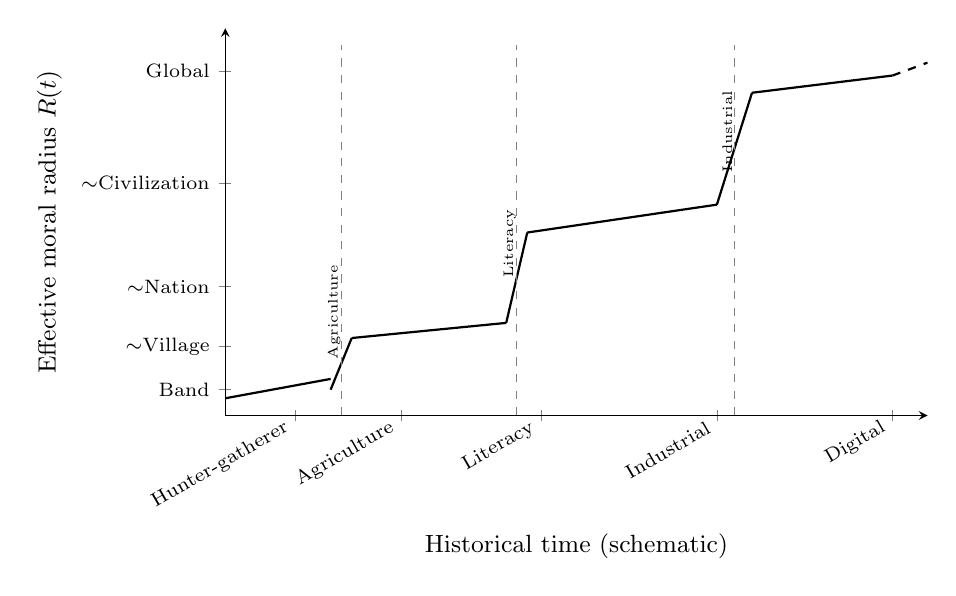
\begin{tikzpicture}
\begin{axis}[
  width=10.5cm, height=6.5cm,
  xlabel={Historical time (schematic)},
  ylabel={Effective moral radius $R(t)$},
  xmin=0, xmax=10,
  ymin=0, ymax=4.5,
  axis lines=left,
  xtick={1,2.5,4.5,7,9.5},
  xticklabels={Hunter-gatherer, Agriculture, Literacy, Industrial, Digital},
  x tick label style={rotate=30, anchor=east, font=\scriptsize},
  ytick={0.3,0.8,1.5,2.7,4.0},
  yticklabels={Band,$\sim$Village,$\sim$Nation,$\sim$Civilization,Global},
  tick label style={font=\scriptsize},
  label style={font=\small},
]

\addplot[thick, black, domain=0:1.5, samples=50]
  {0.2 + 0.15*x};

\addplot[thick, black, domain=1.5:1.8, samples=20]
  {0.3 + 2.0*(x-1.5)};

\addplot[thick, black, domain=1.8:4.0, samples=50]
  {0.9 + 0.08*(x-1.8)};

\addplot[thick, black, domain=4.0:4.3, samples=20]
  {1.076 + 3.5*(x-4.0)};

\addplot[thick, black, domain=4.3:7.0, samples=50]
  {2.126 + 0.12*(x-4.3)};

\addplot[thick, black, domain=7.0:7.5, samples=20]
  {2.45 + 2.6*(x-7.0)};

\addplot[thick, black, domain=7.5:9.5, samples=50]
  {3.75 + 0.10*(x-7.5)};

\addplot[thick, black, dashed, domain=9.5:10, samples=20]
  {3.95 + 0.3*(x-9.5)};

\draw[gray, thin, dashed] (axis cs:1.65,0) -- (axis cs:1.65,4.3);
\draw[gray, thin, dashed] (axis cs:4.15,0) -- (axis cs:4.15,4.3);
\draw[gray, thin, dashed] (axis cs:7.25,0) -- (axis cs:7.25,4.3);

\node[font=\tiny, rotate=90] at (axis cs:1.55,1.2) {Agriculture};
\node[font=\tiny, rotate=90] at (axis cs:4.05,2.0) {Literacy};
\node[font=\tiny, rotate=90] at (axis cs:7.15,3.3) {Industrial};

\end{axis}
\end{tikzpicture}
\caption{Schematic evolution of effective moral radius $R(t)$ under civilizational dynamics. Coordination phase transitions (dashed vertical lines) produce discontinuous expansions in $R(t)$, corresponding to the sudden incorporation of previously distant agents into the scope of recognized solidarity. Between transitions, $R(t)$ grows slowly through gradual diffusion of coordination norms.}
\label{fig:radius}
\end{figure}

\section{Stochastic Institutional Dynamics}
\label{app:stochastic}

Deterministic dynamical systems provide a first approximation to institutional dynamics. A more realistic model incorporates stochastic perturbations arising from individual-level heterogeneity, external shocks, and the intrinsic uncertainty of social processes.

\subsection{Stochastic Differential Equations for Coordination}

Let the institutional state $x(t) \in \mathbb{R}^n$ evolve according to the It\^{o} stochastic differential equation
\[
dx = f(x,t)\,dt + \sigma(x,t)\,dW_t,
\]
where $f : \mathbb{R}^n \times \mathbb{R}_+ \to \mathbb{R}^n$ is the drift field, $\sigma : \mathbb{R}^n \times \mathbb{R}_+ \to \mathbb{R}^{n \times m}$ is the diffusion matrix, and $W_t$ is a standard $m$-dimensional Wiener process.

The drift $f$ captures deterministic coordination pressures, while $\sigma\,dW_t$ models irreducible uncertainty in social dynamics.

\subsection{Fokker--Planck Equation}

The evolution of the probability density $\rho(x,t)$ of the stochastic process is governed by the Fokker--Planck equation
\[
\partial_t \rho = -\nabla \cdot (f\rho) + \frac{1}{2}\sum_{i,j} \partial_{x_i}\partial_{x_j}(D_{ij}\rho),
\]
where $D = \sigma\sigma^T$ is the diffusion tensor. This equation describes how uncertainty propagates through the institutional state space.

\subsection{Stationary Distributions}

A stationary distribution $\rho^*(x)$ satisfies $\partial_t \rho^* = 0$, i.e.,
\[
\nabla \cdot \left(f\rho^* - \tfrac{1}{2}\nabla \cdot (D\rho^*)\right) = 0.
\]

For gradient drift $f = -\nabla V$ and constant isotropic diffusion $D = \varepsilon I$, the stationary distribution takes the Gibbs form
\[
\rho^*(x) = Z^{-1}\exp\!\left(-\frac{2V(x)}{\varepsilon}\right), \qquad Z = \int \exp\!\left(-\frac{2V(x)}{\varepsilon}\right)dx.
\]

In this regime the potential $V$ plays the role of an institutional energy landscape, and $\varepsilon$ quantifies the level of stochastic disruption. As $\varepsilon \to 0$, the stationary distribution concentrates around the global minimum of $V$, recovering the deterministic stable equilibrium.

\subsection{Metastability and Escape from Coordination Regimes}

When $V$ has multiple local minima separated by barriers of height $\Delta V$, the mean escape time from a metastable coordination regime follows the Kramers formula
\[
\mathbb{E}[\tau_{\mathrm{esc}}] \approx C \exp\!\left(\frac{2\Delta V}{\varepsilon}\right),
\]
for some constant $C$ depending on the curvature of $V$ at the minimum and the saddle point. This formula makes precise the intuition that high-performing institutional equilibria can persist despite stochastic perturbations, with stability increasing exponentially in the ratio $\Delta V / \varepsilon$. Civilizational transitions correspond to regimes in which $\Delta V$ decreases---due to technological shock, ecological stress, or informational disruption---to the point where $\mathbb{E}[\tau_{\mathrm{esc}}]$ falls to historically relevant timescales.

\subsection{A Stochastic Stability Theorem}

\begin{theorem}[Stochastic Lyapunov Stability]
Let $dx = f(x)\,dt + \sigma\,dW_t$ with $f = -\nabla V$ and $\sigma$ constant. Suppose $V$ is smooth, positive definite, and radially unbounded. Then for all $\varepsilon > 0$:
\[
\limsup_{t \to \infty} \frac{1}{t} \log \|x(t)\| \le -\frac{\lambda_{\min}(Q)}{\lambda_{\max}(P)}
\]
where $P$ and $Q$ arise from the Lyapunov equation $PA + A^T P = -Q$ for $A = D^2V(0)$.
\end{theorem}

\begin{proof}
The It\^{o} formula applied to $V(x(t))$ yields
\[
dV = \nabla V \cdot f\,dt + \nabla V \cdot \sigma\,dW_t + \tfrac{1}{2}\mathrm{tr}(\sigma^T D^2V\,\sigma)\,dt.
\]
Since $\nabla V \cdot f = -|\nabla V|^2 \le -\lambda_{\min}(D^2V)\|x\|^2$ near the origin and the diffusion term contributes an additive constant, standard stochastic Lyapunov theory (see Khasminskii \cite{khasminskii2012}) yields the exponential stability bound in expectation, from which the almost-sure rate follows by ergodic arguments.
\end{proof}

\section{Topos-Theoretic Coordination}
\label{app:topos}

The sheaf-theoretic framework developed in subsequent appendices can be placed within the broader context of topos theory, which provides the most general setting for treating distributed knowledge and coordination as geometric objects.

\subsection{Grothendieck Topoi}

A Grothendieck topos is a category $\mathcal{E}$ that is equivalent to the category of sheaves on a site $(C, J)$, where $C$ is a small category and $J$ is a Grothendieck topology on $C$.

\begin{definition}
A \emph{site} is a pair $(C, J)$ where $C$ is a category and $J$ assigns to each object $c \in C$ a collection $J(c)$ of \emph{covering sieves} satisfying the axioms of maximality, stability, and transitivity.
\end{definition}

In the context of distributed coordination, we take $C$ to be the poset of coordination contexts ordered by inclusion, and $J(c)$ to be the collection of sieves generated by covering families of agents whose combined information determines the state at $c$. The topos $\mathcal{E} = \sh(C,J)$ then represents the category of all coherent distributed knowledge structures consistent with the coordination topology.

\subsection{Internal Logic and Distributed Reasoning}

Every Grothendieck topos has an associated internal logic---the Mitchell--B\'{e}nabou language---which supports constructive reasoning over distributed information. Propositions in this logic correspond to subobjects of the terminal object $\mathbf{1} \in \mathcal{E}$, and their truth values are elements of the subobject classifier $\Omega$.

\begin{proposition}
In the coordination topos $\mathcal{E} = \sh(C,J)$, the subobject classifier $\Omega$ assigns to each context $c$ the lattice of closed sieves on $c$. A proposition $\phi$ is ``locally true'' at $c$ if it holds on some covering sieve of $c$.
\end{proposition}

This framework provides a precise semantics for distributed epistemic states: an institutional claim is globally valid if and only if it is locally valid on every sufficiently fine cover of the coordination context. This formalization of local-to-global consistency exactly parallels the sheaf gluing conditions developed in Appendix~\ref{app:sheaf}.

\subsection{Geometric Morphisms as Institutional Transformations}

Morphisms between topoi are \emph{geometric morphisms} $f : \mathcal{E} \to \mathcal{F}$, consisting of an adjoint pair $(f^*, f_*)$ with $f^*$ left exact.

\begin{definition}
An institutional transformation from coordination regime $\mathcal{E}$ to regime $\mathcal{F}$ is a geometric morphism $f : \mathcal{E} \to \mathcal{F}$. The inverse image functor $f^* : \mathcal{F} \to \mathcal{E}$ translates coordination structures from the target regime back to the source, while the direct image $f_* : \mathcal{E} \to \mathcal{F}$ pushes forward institutional sections.
\end{definition}

A phase transition in coordination regime corresponds, in this framework, to a change in the underlying site $(C,J)$ and hence to a geometric morphism between the associated topoi. The analysis of such morphisms---in particular, whether they are open, \'{e}tale, or proper---provides a categorical vocabulary for distinguishing gradual institutional adaptation from abrupt structural reorganization.

\subsection{Classifying Topos and Universal Coordination}

For a geometric theory $\mathbb{T}$ (e.g., the theory of a coordination system satisfying certain axioms), there exists a classifying topos $\mathcal{B}\mathbb{T}$ such that models of $\mathbb{T}$ in any topos $\mathcal{E}$ correspond to geometric morphisms $\mathcal{E} \to \mathcal{B}\mathbb{T}$.

In the present context, this means that any specific coordination regime---characterized by its topological structure and institutional logic---can be compared to a universal coordination theory through a canonical geometric morphism. The degree to which this morphism preserves or distorts the institutional logic of $\mathbb{T}$ provides a measure of how well the specific regime approximates the coordination ideal.

\section{Sheaf Structures for Distributed Knowledge}
\label{app:sheaf}

\subsection{Presheaves, Restriction Maps, and Gluing}

Let $X$ be a topological space. A presheaf $\mathcal{F} : \mathcal{O}(X)^{\mathrm{op}} \to \mathbf{Set}$ assigns to each open set $U$ a set $\mathcal{F}(U)$ of locally valid information states, with restriction maps $\rho_{VU} : \mathcal{F}(V) \to \mathcal{F}(U)$ for $U \subseteq V$ satisfying $\rho_{UU} = \mathrm{id}$ and $\rho_{WU} = \rho_{VU} \circ \rho_{WV}$ for $U \subseteq V \subseteq W$.

$\mathcal{F}$ is a \emph{sheaf} if for every open cover $U = \bigcup_i U_i$ and compatible family of sections $s_i \in \mathcal{F}(U_i)$ with $\rho_{U_i, U_i \cap U_j}(s_i) = \rho_{U_j, U_i \cap U_j}(s_j)$, there exists a unique $s \in \mathcal{F}(U)$ with $\rho_{U,U_i}(s) = s_i$.

\subsection{Sheafification}

The sheafification $\mathcal{P} \mapsto \mathcal{P}^{++}$ is the universal construction that forces the gluing condition. Performing the associated-sheaf construction twice---$\mathcal{P} \to \mathcal{P}^+ \to \mathcal{P}^{++}$---produces a sheaf from any presheaf, representing the progressive reconciliation of local knowledge into globally consistent form.

\subsection{Čech Cohomology and Coordination Obstructions}

Given a cover $\mathcal{U} = \{U_i\}$, Čech cochains $\check{C}^k(\mathcal{U},\mathcal{F})$ assign sections to $(k+1)$-fold intersections. The coboundary operator $\delta : \check{C}^k \to \check{C}^{k+1}$ measures local inconsistency, and
\[
H^k(X,\mathcal{F}) = \ker\delta / \mathrm{im}\,\delta
\]
captures global obstructions to coordination. Nontrivial $H^1(X,\mathcal{F})$ indicates topological obstacles to assembling locally consistent information into a global section---a formal analogue of irreducible institutional coordination failure.

\section{Additional Dynamical Structures}

\subsection{Topological and Measure-Theoretic Entropy}

For a compact metric dynamical system $(X,d,T)$, topological entropy is
\[
h_{\mathrm{top}}(T) = \lim_{\varepsilon \to 0}\limsup_{n \to \infty} \tfrac{1}{n}\log N(n,\varepsilon),
\]
where $N(n,\varepsilon)$ is the minimal $(n,\varepsilon)$-cover number under dynamical distance $d_n(x,y) = \max_{0 \le k < n}d(T^k x, T^k y)$. For a measure-preserving system $(X,\mathcal{B},\mu,T)$, the Kolmogorov--Sinai entropy is
\[
h_\mu(T) = \sup_\mathcal{P} \lim_{n \to \infty} \tfrac{1}{n} H_\mu\!\left(\bigvee_{j=0}^{n-1}T^{-j}\mathcal{P}\right).
\]
The variational principle states $h_{\mathrm{top}}(T) = \sup_\mu h_\mu(T)$.

\subsection{Entropy Production in Nonequilibrium Coordination}

For a Fokker--Planck system with flux $J = \rho v - D\nabla\rho$, entropy production rate is
\[
\Pi = \int_X \frac{\|J\|^2}{D\rho}\,dx \ge 0,
\]
with equality only at thermodynamic equilibrium. In coordination contexts, $\Pi$ measures the irreversibility of information processing: a system actively correcting errors and integrating new information necessarily produces positive entropy, a thermodynamic cost of maintaining organized structure against noise.

\subsection{Renormalization and Scale Invariance}

A hierarchy of state spaces $X_0 \xrightarrow{R_0} X_1 \xrightarrow{R_1} \cdots$ with scale-dependent dynamics $T_k : X_k \to X_k$ satisfying $R_k \circ T_k \approx T_{k+1} \circ R_k$ defines a renormalization group. Fixed points $T^* = R(T^*)$ represent scale-invariant coordination structures. The eigenvalues $\nu_i$ of the linearized renormalization operator at $T^*$ determine relevant ($|\nu_i|>1$) and irrelevant ($|\nu_i|<1$) directions, classifying perturbations by whether they grow or decay under successive coarse-graining.

\subsection{Symbolic Dynamics and Coordination Complexity}

The transition matrix $A \in \{0,1\}^{m \times m}$ of a subshift of finite type yields topological entropy $h_{\mathrm{top}}(\Sigma_A) = \log\rho(A)$, connecting coordination complexity directly to spectral properties of the interaction graph. For civilizational coordination, the relevant matrix encodes permissible institutional transitions, and its spectral radius bounds the diversity of achievable coordination trajectories.

\newpage
\begin{thebibliography}{99}

\bibitem{margulis1970}
Lynn Margulis.
\textit{Origin of Eukaryotic Cells}.
Yale University Press, 1970.

\bibitem{margulis1998}
Lynn Margulis and Dorion Sagan.
\textit{What Is Life?}
University of California Press, 1998.

\bibitem{smithszathmary1995}
John Maynard Smith and Eörs Szathmáry.
\textit{The Major Transitions in Evolution}.
Oxford University Press, 1995.

\bibitem{nowak2006}
Martin A. Nowak.
Five Rules for the Evolution of Cooperation.
\textit{Science}, 314(5805):1560--1563, 2006.

\bibitem{kropotkin1902}
Peter Kropotkin.
\textit{Mutual Aid: A Factor of Evolution}.
McClure, Phillips \& Co., 1902.

\bibitem{ostrom1990}
Elinor Ostrom.
\textit{Governing the Commons: The Evolution of Institutions for Collective Action}.
Cambridge University Press, 1990.

\bibitem{henrich2016}
Joseph Henrich.
\textit{The Secret of Our Success: How Culture Is Driving Human Evolution}.
Princeton University Press, 2016.

\bibitem{turchin2016}
Peter Turchin.
\textit{Ultrasociety: How 10,000 Years of War Made Humans the Greatest Cooperators on Earth}.
Beresta Books, 2016.

\bibitem{shannon1948}
Claude E. Shannon.
A Mathematical Theory of Communication.
\textit{Bell System Technical Journal}, 27:379--423, 623--656, 1948.

\bibitem{hanson1958}
Norwood Russell Hanson.
\textit{Patterns of Discovery: An Inquiry into the Conceptual Foundations of Science}.
Cambridge University Press, 1958.

\bibitem{kuhn1962}
Thomas S. Kuhn.
\textit{The Structure of Scientific Revolutions}.
University of Chicago Press, 1962.

\bibitem{smolin2013}
Lee Smolin.
\textit{Time Reborn: From the Crisis in Physics to the Future of the Universe}.
Houghton Mifflin Harcourt, 2013.

\bibitem{wilson2012}
Edward O. Wilson.
\textit{The Social Conquest of Earth}.
W. W. Norton \& Company, 2012.

\bibitem{strogatz2001}
Steven H. Strogatz.
\textit{Nonlinear Dynamics and Chaos}.
Perseus Books, 2001.

\bibitem{thom1975}
René Thom.
\textit{Structural Stability and Morphogenesis}.
W. A. Benjamin, 1975.

\bibitem{golubitsky1985}
Martin Golubitsky and David G. Schaeffer.
\textit{Singularities and Groups in Bifurcation Theory}, vol.~1.
Springer-Verlag, 1985.

\bibitem{mackay2003}
David J. C. MacKay.
\textit{Information Theory, Inference, and Learning Algorithms}.
Cambridge University Press, 2003.

\bibitem{olfatisaber2007}
Reza Olfati-Saber, J.~Alex Fax, and Richard M. Murray.
Consensus and Cooperation in Networked Multi-Agent Systems.
\textit{Proceedings of the IEEE}, 95(1):215--233, 2007.

\bibitem{amari2000}
Shun-ichi Amari and Hiroshi Nagaoka.
\textit{Methods of Information Geometry}.
American Mathematical Society, 2000.

\bibitem{sga4}
Michael Artin, Alexander Grothendieck, and Jean-Louis Verdier.
\textit{Théorie des Topos et Cohomologie Étale des Schémas} (SGA 4).
Springer-Verlag, 1972.

\bibitem{maclanemoerdijk}
Saunders Mac Lane and Ieke Moerdijk.
\textit{Sheaves in Geometry and Logic: A First Introduction to Topos Theory}.
Springer-Verlag, 1992.

\bibitem{walters2000}
Frederick Walters.
\textit{An Introduction to Ergodic Theory}.
Springer-Verlag, 2000.

\bibitem{khasminskii2012}
Rafail Khasminskii.
\textit{Stochastic Stability of Differential Equations}, 2nd ed.
Springer-Verlag, 2012.

\bibitem{hofbauersigmund1998}
Josef Hofbauer and Karl Sigmund.
\textit{Evolutionary Games and Population Dynamics}.
Cambridge University Press, 1998.

\bibitem{risken1989}
Hannes Risken.
\textit{The Fokker--Planck Equation: Methods of Solution and Applications}, 2nd ed.
Springer-Verlag, 1989.

\end{thebibliography}

\end{document}
